\documentclass [11pt, a4wide, twoside]{article}

\usepackage{times}
\usepackage{epsfig}
\usepackage{ifthen}
\usepackage{xspace}
\usepackage{fancyhdr}
\usepackage{moreverb}
\usepackage{amsmath}
\usepackage{hyperref} % for figures
\usepackage{listings} % for Java code
\usepackage{color} % for Java code

%========================JAVA CODE========================
\definecolor{source}{gray}{0.9}
\lstset{
	% characters
	tabsize=3,
	upquote=true, % straight quote; requires textcomp package
	escapechar={!},
	keepspaces=true,
	breaklines=false,
	alsoletter={:},
	breakautoindent=true,
	columns=fullflexible,
	showspaces=false,
	showstringspaces=false,
	basicstyle=\small\ttfamily,
	% background
	frame=single,
   	framerule=0pt,
	backgroundcolor=\color{source},
	% numbering
	numbersep=10pt,
	stepnumber=1,
	numberstyle=\tiny,
	numberfirstline=true,
	% captioning
	captionpos=b,
	numberbychapter=false}
\definecolor{javared}{rgb}{0.6,0,0} % for strings
\definecolor{javagreen}{rgb}{0.25,0.5,0.35} % comments
\definecolor{javapurple}{rgb}{0.5,0,0.35} % keywords
\definecolor{javadocblue}{rgb}{0.25,0.35,0.75} % javadoc
%Java listing
\lstdefinestyle{Java}{
	language=Java,
	keywordstyle=\color{javapurple}\bfseries,
	stringstyle=\color{javared},
	commentstyle=\color{javagreen},
	morecomment=[s][\color{javadocblue}]{/**}{*/}
}
\newcommand{\jlct}{\lstinline[backgroundcolor=\color{white},style=Java]}
%========================================================

% solution switch
\newboolean{showsolution}
%\setboolean{showsolution}{true}
\setboolean{showsolution}{true}



%layout
\topmargin      -5.0mm
\oddsidemargin  6.0mm
\evensidemargin -6.0mm
\textheight 215.5mm
\textwidth      160.0mm
\parindent        1.0em
\headsep          10.3mm
\headheight        12pt
\lineskip    1pt
\normallineskip     1pt

%header
\lhead{Programming Languages \\ 2021}

\rhead{Prof. O. Nierstrasz\\
Mohammadreza Hazhirpasand, Joel Niklaus}
\lfoot{page \thepage}
\rfoot{\today}
\cfoot{}

\renewcommand{\headrulewidth}{0.1pt}
\renewcommand{\footrulewidth}{0.1pt}

\renewcommand{\thesubsection}{\arabic{subsection}}

%enumeration
\newenvironment{myitemize}{%
     \begin{itemize}
     \setlength{\itemsep}{0cm}}
     {\end{itemize}}

\newenvironment{myenumerate}{%
     \begin{enumerate} \setlength{\itemsep}{0cm}}
     {\end{enumerate}}


%solution
\ifthenelse{\boolean{showsolution}}
   {  \newcommand{\solution}[1]{
   	\noindent\underline{\textbf{Answer:}}\\[2mm]
   	 \textsl{#1}
	 \vspace{10pt}
	 \normalsize
	}
  }
  {  \newcommand{\solution}[1]{} }

\newcounter{exnum}
\def\xexercise{\fontsize{12}{10}\fontseries{bx}\selectfont}
\def\xnormal{\fontseries{m}\fontshape{n}\selectfont}


\newcommand{\exercise}[1]{%
     {\addtocounter{exnum}{1}\vskip 0.8cm{\xexercise \noindent Exercise
\arabic{exnum} (#1)} \xnormal} \vskip 0.3cm} 
 \newcommand{\aufgabe}[1]{
     {\addtocounter{exnum}{1}\vskip 0.8cm{\xexercise \noindent Aufgabe
\arabic{exnum} (#1)} \xnormal} \vskip 0.3cm} 

\pagestyle{fancy}


% ===============ABBREVIATIONS==============================
\newcommand{\eg}{\emph{e.g.,}\xspace}
\newcommand{\ie}{\emph{i.e.,}\xspace}
\newcommand{\etc}{\emph{etc.}\xspace}


\begin{document}

% title
\section*{
    \ifthenelse{\boolean{showsolution}}{Solution }{}
    \xspace{}Serie 9 - Objects and Types}

%==============================================================================
\subsection{Theoretical Questions (6 points)}

\begin{myenumerate}

\item What is the difference between subtyping and subclassing? Provide an example for your explanation.

\vspace{0.5cm}

\solution{Substitution (subtype) ��a specification notion. B is a subtype of A if an object of B can masquerade as an object of A in any context.

Inheritance (subclass)�� should not be confused with subtyping. In general, subtyping establishes an is-a
relationship, whereas subclassing only reuses implementation and establishes a syntactic relationship,
not necessarily a semantic relationship (inheritance does not ensure behavioral subtyping). 

To distinguish these concepts, subtyping is also known as interface inheritance, whereas subclassing is
known as implementation inheritance or code inheritance. Subclassing example is in question number 4. }


\item Using the Java class-interface hierarchy given in \autoref{fig:hierarchy}, explain what is the relationship between classes and interfaces.

\begin{figure}[h!]
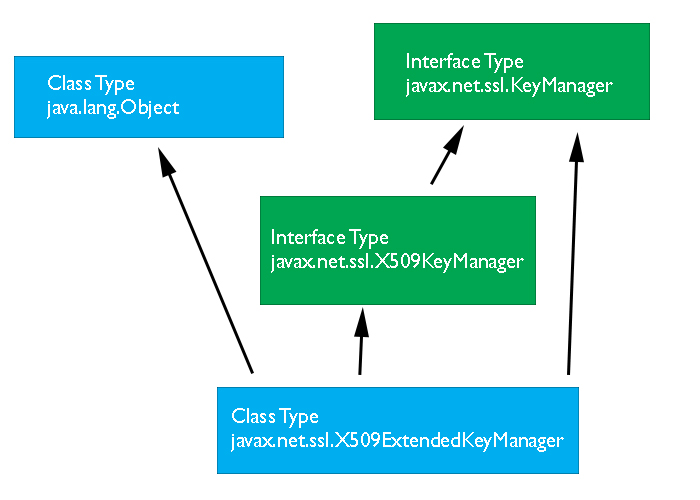
\includegraphics[width=0.5\linewidth]{figs/hierarchy.jpg}
\caption{Java interface hierarchy}
\label{fig:hierarchy}
\end{figure}

\vspace{0.5cm}

\solution{\texttt{javax.net.ssl.X509ExtendedKeyManager} is a subtype of \texttt{java.lang.Object.}

\texttt{javax.net.ssl.X509ExtendedKeyManager} is a subtype of \texttt{javax.net.ssl.X509KeyManager}.

\texttt{javax.net.ssl.X509ExtendedKeyManager} is a subtype of \texttt{javax.net.ssl.KeyManager}.

\texttt{javax.net.ssl.KeyManager} is a supertype of \texttt{javax.net.ssl.X509ExtendedKeyManager}.

\texttt{javax.net.ssl.KeyManager} is a supertype of \texttt{javax.net.ssl.X509KeyManager}.

\texttt{java.lang.Object} is a supertype of all other class and interface types.}

\item Which forms of polymorphism are used in the Java code in \autoref{lst:poly}? Explain each of the forms.

\begin{lstlisting}[float=h,style=Java,caption={Forms of polymorphism},label=lst:poly]
public class Bern<TT> { // Hint 2
    private TT var1;
    public void set(TT mh) { this.var1 = mh; }
    public TT get() { return var1; }

 public static void main(String[] args) {
 	int a = 3;
	float b = 2F;
	b = a;   // Hint 1
	System.out.println(b);
	Bern<Integer> mj = new Bern();
	mj.set(12);
	System.out.println(mj.get());
	}
}
\end{lstlisting}

\solution{Hint 1: Coercion  \\
Hint 2: Parametric Polymorphism}

\item Use Java subclassing to better structure the code in \autoref{lst:subclassing} and avoid code cloning.

\begin{lstlisting}[float=t,style=Java,caption={Subclassing},label=lst:subclassing]
	class Bicycle {
		private int frame_size;
		
		// the price of this bicycle
		public float price() { return 100 * 2; }

		// the sales tax on this bicycle
		public float salesTax() { return price() * .08; }
}

	class RacingBicycle {
		private int frame_size;
		private int pieces_count;

		// the price of this bicycle
		public float price() { return 100 * 2; }

		// the sales tax on this bicycle
		public float salesTax() { return price() * .08; }

		// returns the weight of this bicycle
		public void calculateWeight();
}
\end{lstlisting}

\solution{\begin{verbatim}
class Bicycle {
private int frame_size;
public float price() { return 100 * 2; }
public float salesTax() { return price() * .08; }
}
class RacingBicycle extends Bicycle {
private int pieces_count;
public void calculateWeight();

}
\end{verbatim}
}

\item In the code in \href{http://scg.unibe.ch/download/lectures/pl2018-exercises/q5.zip}{q5.zip} explain how covariant and contravariant are used in each code block. Why are there compile-time errors if you try to run the code?
\end{myenumerate}

\solution{Covariance \\ 

In Java, Arrays are covariant. an array of type T[] can store array of subtype S[], which means accepting subtypes.\\
In the example, the supertype (Number) can accept the subtype (Integer).\\
}

\end{document}

